% This is samplepaper.tex, a sample chapter demonstrating the
% LLNCS macro package for Springer Computer Science proceedings;
% Version 2.20 of 2017/10/04
%
\documentclass[runningheads]{llncs}
%
\usepackage{graphicx}
\usepackage[utf8x]{inputenc}
\usepackage[ampersand]{easylist}
\usepackage{graphicx}
% Used for displaying a sample figure. If possible, figure files should
% be included in EPS format.
%
% If you use the hyperref package, please uncomment the following line
% to display URLs in blue roman font according to Springer's eBook style:
% \renewcommand\UrlFont{\color{blue}\rmfamily}

\begin{document}
%
\title{Conversation-Based Complex Event Management in Smart-Spaces}
%\title{Exploring Complex Event Management
%in Smart-Spaces through a
%Conversation-Based Approach}
%
\titlerunning{Conversation-Based Complex Event Management in Smart-Spaces}
% If the paper title is too long for the running head, you can set
% an abbreviated paper title here
%
\author{André Sousa Lago\inst{1}\orcidID{0000-0002-4534-9180} \and
Hugo Sereno Ferreira\inst{2}\orcidID{0000-0002-4963-3525}}
% \author{First Author\inst{1}\orcidID{0000-1111-2222-3333} \and
% Second Author\inst{2,3}\orcidID{1111-2222-3333-4444} \and
% Third Author\inst{3}\orcidID{2222--3333-4444-5555}}
%
\authorrunning{André S. Lago, Hugo S. Ferreira}
% First names are abbreviated in the running head.
% If there are more than two authors, 'et al.' is used.
%
\institute{Faculty of Engineering of University of Porto, 4200-465 Porto, Portugal \and
Department of Informatics Engineering, Faculty of Engineering of University of Porto, 4200-465 Porto, Portugal}
%
\maketitle              % typeset the header of the contribution
%
\begin{abstract}
    Smart space management can be done in many ways. On one hand, there are conversational assistants such as the Google Assistant or Amazon Alexa that enable users to comfortably interact with smart spaces with only their voice, but these have limited functionality and are usually limited to simple commands. On the other hand, there are visual interfaces such as IBM's Node-RED that enable complex features and dependencies between different devices. However, these are limited since they require users to have a technical knowledge of how the smart devices work and the system's interface is more complicated and harder to use since they require a computer.
    This project proposes a new conversational assistant - Jarvis - that combines the ease of use of current assistants with the operational complexity of the visual platforms. The goal of Jarvis is to make it easier to manage smart spaces by providing intuitive commands and useful features. Jarvis integrates with already existing user interfaces such as the Google Assistant, Slack or Facebook Messenger, making it very easy to integrate with existing systems. Jarvis also provides an innovative feature - causality queries - that enable users to ask it why something happened. For example, a user can ask "\textit{why did the light turn on?}" to understand how the system works.

\keywords{Human-centered computing → Natural language interfaces.}
\end{abstract}
%
%
%
\section{Introduction}

\subsection{Internet of Things}

The Internet of Things, or IoT, is the networked connection of everyday objects, which is often equipped with a collective sense of intelligence~\cite{Xia2012}. The integration of such objects creates a huge range of distributed systems that are able to interact with the environment and human beings around them in a lot of different ways.

The flexibility of IoT systems has enabled their use across many different product areas and markets, including smart homes, smart cities, healthcare, transportation, retail, wearables, agriculture and industry~\cite{Rahul2017}.

IoT is a booming technological market, and Gartner predicts that 11.2 billion devices will be connected in 2018, a number that is also predicted to almost double over the following 2 years, becoming 20.4 billion devices by 2020~\cite{VanderMeulen2017}. The Boston Consulting Group also estimates that by 2020 companies will spend 250 billion Euros in IoT on top of what they already spend on other technologies~\cite{Hunke2017}. This means that not only more people will be using IoT, but also that it will be present in a lot of different environments and situations. This represents a unique opportunity for IoT to evolve as a facilitator on people’s lives. After all, having intelligently connected devices around us should help us make our day to day lives easier.

This boom in worldwide connected devices has led to a lot of different applications of these technologies across countries and product areas. Although being a relatively small sample, the examples below demonstrate different use cases of IoT when combined with multiple technologies and markets~\cite{Chen2014,Lee2015,Xu2014}.

\textbf{Smart Homes} are the IoT application of domotics. While domotics usually refers to individual systems that perform isolated tasks automatically, smart homes usually refer to a set of connected sensors and electronics that allow for a house to be more autonomous. Some smart houses include appliances such as fridges that remind users when a certain item is about to run out, self-regulating temperature systems or self-locking door and window mechanisms. Perhaps more importantly, many of these devices can be controlled or monitored remotely which provides users with a greater sense of control of their appliances.

\textbf{Wearables} are devices that are worn like clothes, accompanying human beings in their regular activities. Some examples of wearable devices are smartwatches, step counters or smart glasses. With the sizes of processors and electronic boards shrinking, the capabilities of these devices have increased, and such can be seen in the growth of this industry segment which was predicted to surpass 4 billion dollars in 2017 by Forbes~\cite{Marr2016}.

\textbf{Smart Cities} are a concept similar to smart homes, where the same technology is applied in the context of a public space. These usually aim towards simplifying urban life, or making it more environment-friendly. The most common use cases in this segment are smart parking spaces, smart waste management systems or smart street lighting.

\textbf{Retail} can also be an interesting use case for IoT as it can benefit both customers and store managers. In these cases, IoT can not only help customers instantly know whether a certain product is in stock or not, but also help the manager determine when to order a certain product based on its current shelf stock.

\textbf{Healthcare} is yet another field where IoT can be very beneficial, as it can help doctors remotely keep track of a patient’s live status, or receive an alert when a problem is detected with a patient. An article by IBM even alerts that even though there are a lot of problems around IoT in healthcare, especially due to data privacy, it can help reduce healthcare costs or improve the outcome of treatments~\cite{Patel2017}.

Finally, \textbf{customized smart spaces} are a logical consequence of the growth of IoT and its associated products, as it became possible for almost everyone to create a customized IoT experience based on products and hardware available. In any IoT system, the essential items are the physical devices that are connected by the system and interact with the environment. In this document these are called \textbf{leaf devices}. 

The first step to create a customized smart space is to acquire the leaf devices, depending on the intended use for the system. Some of the most common leaf devices are temperature sensors, motion sensors and remote light switches.

Although some of these devices have controllers of their own that can be programmed or controlled in a certain way, it is also possible to acquire \textbf{middleware devices} that connect to the leaf devices, and therefore are able to read and modify their current status. 

Arduino boards and Raspberry Pi computers, which were mentioned above, are often used as middleware devices due to their setup simplicity and low cost. For example, a Raspberry Pi’s GPIO\footnote{General Purpose Input/Output, multi-purpose ports that can be programmed for different inputs and outputs} ports can be simultaneously connected to a luminosity sensor and a light switch. That way, not only the luminosity value of the sensor can be sent to a remote server via Wi-Fi, but also the light switch can be turned on when the luminosity drops below a certain level. Arduino boards can also be used to increase the capacity of simpler devices such as sensors or actuators. For example, an Arduino board can be connected to a sensor providing it with a connection to a local network, so that the sensor’s status can be accessed remotely.

Once the devices are acquired, it is necessary to connect them to a network and manage their behavior. To achieve this, a common technique is to use a \textbf{supervisor device}, a middleware device that acts as a supervisor for all the other devices. A computer or Raspberry Pi are common supervisor devices as these usually require a bit more power than alternatives like Arduino boards can offer. Once the supervisor device is ready, platforms like Node-RED\footnote{\url{https://nodered.org/}} or Home Assistant\footnote{\url{https://home-assistant.io/}} can be installed to facilitate the management of the system as a whole. These \textbf{management platforms} are described thoroughly below.

As a practical example, let’s picture a user that wants to have a luminosity sensor and a temperature sensor in his room, and an actuator that can open and close the window. With these, the user wants to have a dashboard where he can consult the history of the room’s luminosity as well as the status (open/closed) of the window. Finally, the user wants the window to be shut if the temperature drops below a certain level. To achieve this functionality, all the user needs is to buy the actual sensors, the actuator and a Raspberry Pi. Then, the sensors and the actuator are connected to the Pi, which is then given an installation of Node-RED, so that the user can make the window close when the temperature drops.

\subsection{Visual Programming Paltforms}
\subsection{Conversational Assistants}
\subsection{IoT Communication Protocols}

\section{Problem Statement}
\subsection{Current Issues}
\subsection{Proposal}
\subsection{Desiderata}
\subsection{Research Questions}

\section{Developed Solution}
\subsection{Proposed Features}
\subsection{Software Components}

\section{Validation}
\subsection{Simulated Scenarios}
\subsection{User Study}

\section{Conclusions and Future Work}

\begin{table}
    \caption{User Study results (task completion rate, task time and incorrect queries).}
    \centering
    \begin{tabular}{ | c | c | c | c | c | c | c | c | c | c | c | c |}
    \hline
    \multicolumn{2}{|c|}{} & \multicolumn{2}{|c|}{Time} & \multicolumn{2}{|c|}{IQ (Ast)} & \multicolumn{2}{|c|}{IQ (User)} & \multicolumn{2}{|c|}{IQ (Jvs)} & \multicolumn{2}{|c|}{IQ} \\ \hline
    Task & Done & Avg & Med & Avg & Med & Avg & Med & Avg & Med & Avg & Med \\ \hline
    
    0 (1) & 94\% & 6.4 & 6 & 0.13 & 0 & 0.25 & 0 & 0.13 & 0 & 0.5 & 0 \\ \hline
    1 (1) & 94\% & 7.1 & 7 & 0.38 & 0 & 0.5 & 0.5 & 0 & 0 & 0.5 & 0.5 \\ \hline
    2 (1) & 88\% & 10 & 10 & 0.75 & 0.5 & 0.63 & 0.5 & 0.25 & 0 & 1 & 1 \\ \hline
    3 (1) & 100\% & 20 & 19.5 & 0.13 & 0 & 0.13 & 0 & 0.75 & 1 & 1 & 1 \\ \hline
    4 (1) & 94\% & 9 & 8 & 0.25 & 0 & 0.38 & 0 & 0 & 0 & 0.63 & 0 \\ \hline
    0 (2) & 100\% & 6.4 & 6 & 0.33 & 0 & 0 & 0 & 0.33 & 0 & 0.67 & 0 \\ \hline
    1 (2) & 94\% & 7.6 & 7 & 0.11 & 0 & 0 & 0 & 0.44 & 0 & 0.56 & 0 \\ \hline
    2 (2) & 100\% & 9.9 & 10 & 0 & 0 & 0.11 & 0 & 0.78 & 1 & 0.89 & 1 \\ \hline
    3 (2) & 88\% & 19.44 & 19 & 0.33 & 0 & 0.33 & 0 & 0.22 & 0 & 0.89 & 1 \\ \hline
    4 (2) & 100\% & 8.33 & 8 & 0.33 & 0 & 0.22 & 0 & 0.22 & 0 & 0.78 & 1 \\ \hline
    \end{tabular}

    \label{table:studyresults}
\end{table}

\section{First Section}
\subsection{A Subsection Sample}
Please note that the first paragraph of a section or subsection is
not indented. The first paragraph that follows a table, figure,
equation etc. does not need an indent, either.

Subsequent paragraphs, however, are indented.

\subsubsection{Sample Heading (Third Level)} Only two levels of
headings should be numbered. Lower level headings remain unnumbered;
they are formatted as run-in headings.

\paragraph{Sample Heading (Fourth Level)}
The contribution should contain no more than four levels of
headings. Table~\ref{tab1} gives a summary of all heading levels.

\begin{table}
\caption{Table captions should be placed above the
tables.}\label{tab1}
\begin{tabular}{|l|l|l|}
\hline
Heading level &  Example & Font size and style\\
\hline
Title (centered) &  {\Large\bfseries Lecture Notes} & 14 point, bold\\
1st-level heading &  {\large\bfseries 1 Introduction} & 12 point, bold\\
2nd-level heading & {\bfseries 2.1 Printing Area} & 10 point, bold\\
3rd-level heading & {\bfseries Run-in Heading in Bold.} Text follows & 10 point, bold\\
4th-level heading & {\itshape Lowest Level Heading.} Text follows & 10 point, italic\\
\hline
\end{tabular}
\end{table}


\noindent Displayed equations are centered and set on a separate
line.
\begin{equation}
x + y = z
\end{equation}
Please try to avoid rasterized images for line-art diagrams and
schemas. Whenever possible, use vector graphics instead (see
Fig.~\ref{fig1}).

\begin{figure}
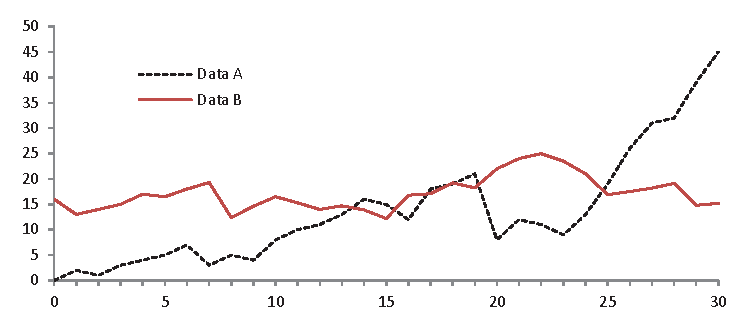
\includegraphics[width=\textwidth]{fig1.eps}
\caption{A figure caption is always placed below the illustration.
Please note that short captions are centered, while long ones are
justified by the macro package automatically.} \label{fig1}
\end{figure}

\begin{theorem}
This is a sample theorem. The run-in heading is set in bold, while
the following text appears in italics. Definitions, lemmas,
propositions, and corollaries are styled the same way.
\end{theorem}
%
% the environments 'definition', 'lemma', 'proposition', 'corollary',
% 'remark', and 'example' are defined in the LLNCS documentclass as well.
%
\begin{proof}
Proofs, examples, and remarks have the initial word in italics,
while the following text appears in normal font.
\end{proof}
% For citations of references, we prefer the use of square brackets
% and consecutive numbers. Citations using labels or the author/year
% convention are also acceptable. The following bibliography provides
% a sample reference list with entries for journal
% articles~\cite{ref_article1}, an LNCS chapter~\cite{ref_lncs1}, a
% book~\cite{ref_book1}, proceedings without editors~\cite{ref_proc1},
% and a homepage~\cite{ref_url1}. Multiple citations are grouped
% \cite{ref_article1,ref_lncs1,ref_book1},
% \cite{ref_article1,ref_book1,ref_proc1,ref_url1}.
%
% ---- Bibliography ----
%
% BibTeX users should specify bibliography style 'splncs04'.
% References will then be sorted and formatted in the correct style.
%
\bibliographystyle{splncs04}
\bibliography{mybibliography}
%
%\begin{thebibliography}{8}
% \bibitem{ref_article1}
% Author, F.: Article title. Journal \textbf{2}(5), 99--110 (2016)

% \bibitem{ref_lncs1}
% Author, F., Author, S.: Title of a proceedings paper. In: Editor,
% F., Editor, S. (eds.) CONFERENCE 2016, LNCS, vol. 9999, pp. 1--13.
% Springer, Heidelberg (2016). \doi{10.10007/1234567890}

% \bibitem{ref_book1}
% Author, F., Author, S., Author, T.: Book title. 2nd edn. Publisher,
% Location (1999)

% \bibitem{ref_proc1}
% Author, A.-B.: Contribution title. In: 9th International Proceedings
% on Proceedings, pp. 1--2. Publisher, Location (2010)

% \bibitem{ref_url1}
% LNCS Homepage, \url{http://www.springer.com/lncs}. Last accessed 4
% Oct 2017

% END OF SAMPLES

% \bibitem{XYWV12}
% Xia, F., Yang, L. T., Wang, L., Vinel, A. (2012). Internet of Things. INTERNATIONAL JOURNAL OF COMMUNICATION SYSTEMS Int. J. Commun. Syst. Int. J. Commun. Syst, 25(25). https://doi.org/10.1002/dac

%\end{thebibliography}
\end{document}

% Dorri, A., Kanhere, S. S., Jurdak, R., & Gauravaram, P. (2017). Blockchain for IoT security and privacy: The case study of a smart home. In 2017 IEEE International Conference on Pervasive Computing and Communications Workshops (PerCom Workshops) (pp. 618–623). IEEE. https://doi.org/10.1109/PERCOMW.2017.7917634
% Techlabs, M. (2017). Exploring Dialogflow: Understanding Agent Interaction. Retrieved from https://chatbotslife.com/which-are-the-best-on-site-chatbot-frameworks-3dbf5157fb57
% Davydova, O. (2017). 25 Chatbot Platforms: A Comparative Table. Retrieved from https://chatbotsjournal.com/25-chatbot-platforms-a-comparative-table-aeefc932eaff
% Birch, J. (2017). Exploring Dialogflow: Understanding Agent Interaction. Retrieved from https://medium.com/@hitherejoe/exploring-dialogflow-understanding-agent-interaction-8f3323e3b738
% Apache. (2005, June). Batik \svg{} {T}oolkit {A}rchitecture.
% Apache. (2005, June). Batik {SVG} {T}oolkit.
% Lipsum. (2008). Lorem Ipsum.
% Tham, M. (2001, May). Writing Research Theses or Dissertations.
% Marinho, F., Viegas, P., & Lopes, J. C. (2006). {SVG} na Visualização de Sinópticos. In J. C. Ramalho, J. C. Lopes, & A. Simões (Eds.), {XATA2006}, XML: Aplicações e Tecnologias Associadas (Portalege, 9 e 10 de Fevereiro de 2006) (pp. 99–112). Universidade do Minho.
% Zukowski, D. J., Purakayastha, A., Mohindra, A., & Devarakonda, M. (1997). Metis: A Thin-Client Application Framework. Proceedings of the Third Conference on Object-Oriented Technologies and Systems, 103–114.
% Matos, M. A. (1993). Normas para Apresentação de Dissertações, Bases Essenciais.
% Franz, M. S. O. (1995). Code-Generation On-the-Fly: A Key to Portable Software. Swiss Federal Institute of Technology Zurich, ETH Zürich.
% Randall, D. (2003). Living inside a smart home: A case study. In Inside the smart home (pp. 227–246). Springer.
% Griss, M. L. (1997). Software reuse architecture, process, and organization for business success. In Proceedings of the Eighth Israeli Conference on Computer Systems and Software Engineering. IEEE Comput. Soc. https://doi.org/10.1109/ICCSSE.1997.599879
% Hertzfeld, A. (1984). It Sure Is Great To Get Out Of That Bag! Folklore. Retrieved from https://www.gartner.com/newsroom/id/2905717
% Chowdhury, G. G. (2003). Natural language processing. Annual Review of Information Science and Technology, 37(1). https://doi.org/10.1002/aris.1440370103
% Allan, D. (2017). The best voice recognition software of 2017. TechRadar. Retrieved from http://www.techradar.com/news/the-best-voice-recognition-software-of-2017
% Juang, B. H., & Rabiner, L. R. (2004). Automatic Speech Recognition – A Brief History of the Technology Development. Retrieved from http://www.ece.ucsb.edu/Faculty/Rabiner/ece259/Reprints/354_LALI-ASRHistory-final-10-8.pdf
% Patel, K. (2017). 6 Benefits of Internet of Things for Hospitals and Healthcare. IBM. Retrieved from https://www.ibm.com/blogs/internet-of-things/6-benefits-of-iot-for-healthcare/
% Marr, B. (2016). 15 noteworthy facts about Wearables in 2016. Forbes. Retrieved from https://www.forbes.com/sites/bernardmarr/2016/03/18/15-mind-boggling-facts-about-wearables-in-2016/#79ad0f5e2732
% Xu, L. Da, He, W., & Li, S. (2014, November). Internet of things in industries: A survey. IEEE Transactions on Industrial Informatics. https://doi.org/10.1109/TII.2014.2300753
% Lee, I., & Lee, K. (2015). The Internet of Things (IoT): Applications, investments, and challenges for enterprises. Business Horizons, 58(4), 431–440. https://doi.org/10.1016/j.bushor.2015.03.008
% Chen, S., Xu, H., Liu, D., Hu, B., & Wang, H. (2014). A vision of IoT: Applications, challenges, and opportunities with China Perspective. IEEE Internet of Things Journal. https://doi.org/10.1109/JIOT.2014.2337336
% Rivera, J., & van der Meulen, R. (2014). Gartner Says 4.9 Billion Connected “Things” Will Be in Use in 2015. Gartner - Newsroom, 9–10. https://doi.org/10.1017/CBO9781107415324.004
% Brown, P. (2017). 20 Billion Connected Internet of Things Devices in 2017, IHS Markit Says. Electronics360. Retrieved from http://electronics360.globalspec.com/article/8032/20-billion-connected-internet-of-things-devices-in-2017-ihs-markit-says
% Dennis, A. K. (2013). Raspberry Pi home automation with Arduino. Packt Publishing Ltd.
% Deering, S. E. (1998). Internet protocol, version 6 (IPv6) specification.
% Sean Dodson. (2003). The internet of things. The Guardian. Retrieved from https://www.theguardian.com/technology/2003/oct/09/shopping.newmedia
% Florea, A., & Sgârciu, V. (2016). Smart refrigerator : A next generation refrigerator connected to the IoT. In Proceedings of the 8th International Conference on Electronics, Computers and Artificial Intelligence, ECAI 2016 (pp. 1–6). IEEE. https://doi.org/10.1109/ECAI.2016.7861170
% Kevin Ashton. (2009). That “Internet of Things” Thing. RFID Journal. Retrieved from http://www.rfidjournal.com/articles/view?4986
% Suresh, P., Daniel, J. V., Parthasarathy, V., & Aswathy, R. H. (2014). A state of the art review on the Internet of Things (IoT) history, technology and fields of deployment. In 2014 International Conference on Science Engineering and Management Research (ICSEMR). IEEE. https://doi.org/10.1109/ICSEMR.2014.7043637
% 1.5 Million Home Automation Systems Installed in the US This Year. (2012). Retrieved from https://www.abiresearch.com/press/15-million-home-automation-systems-installed-in-th/
% Average hours per day spent in selected activities by sex and day. (2017). Bureau of Labor Statistics. Retrieved from https://www.bls.gov/charts/american-time-use/activity-by-sex.htm
% Dr. Brian M. Pierce. (n.d.). Autonomous Real-time Ground Ubiquitous Surveillance - Infrared (ARGUS-IR). DARPA. Retrieved from https://www.darpa.mil/program/autonomous-real-time-ground-ubiquitous-surveillance-infrared
% Peterson, H. (2017). How automation will impact the retail industry. Business Insider. Retrieved from http://www.businessinsider.com/how-automation-will-impact-the-retail-industry-2017-5
% Oliver Balch. (2017). Automated mining will cost jobs and tax income: it’s time for governments to act. The Guardian. Retrieved from https://www.theguardian.com/sustainable-business/2017/jan/20/autonomous-mining-will-cost-jobs-and-tax-income-its-time-for-governments-to-act
% McFarland, M. (2017). Why Volvo’s self-driving garbage truck spends most of its time in reverse. Retrieved from http://money.cnn.com/2017/05/18/technology/volvo-garbage-truck/index.html
% Musson, A. E., & Robinson, E. (1969). Science and technology in the industrial revolution. Manchester University Press.
% Jerome, H. (1934). Mechanization in Industry. National Bureau of Economic Research, 158.
% Guarnieri, M. (2010). The roots of automation before mechatronics. In IEEE Industrial Electronics Magazine (Vol. 4, pp. 42–43). https://doi.org/10.1109/MIE.2010.936772
% ISA. (2010). What is Automation? - ISA. Isa. Retrieved from https://www.isa.org/about-isa/what-is-automation/
% Santos, J., Rodrigues, J. J. P. C., Casal, J., Saleem, K., & Denisov, V. (2016). Intelligent Personal Assistants Based on Internet of Things Approaches. IEEE Systems Journal, 1–10. https://doi.org/10.1109/JSYST.2016.2555292
% Hunke, N., Rüßmann, M., Schmieg, F., Bhatia, A., & Kalra, N. (2017). Winning in IoT: It’s All About the Business Processes. Bgc.perspectives. Retrieved from https://www.bcg.com/publications/2017/hardware-software-energy-environment-winning-in-iot-all-about-winning-processes.aspx
% van der Meulen, R. (2017). Gartner Press Release, Gartner Says 8.4 Billion Connected “Things” Will Be in Use in 2017, Up 31 Percent From 2016. Gartner Press Release. https://doi.org/10.1017/CBO9781107415324.004
% Rasch, K. (2014). An unsupervised recommender system for smart homes. Journal of Ambient Intelligence and Smart Environments, 6, 21–37. https://doi.org/10.3233/AIS-130242
% 
% Mourya, R. (2017). IoT applications spanning across industries. IBM. Retrieved from https://www.ibm.com/blogs/internet-of-things/iot-applications-industries/
% García, R. G. (2005). \svg{} for {SCADA}.
% World Wide Web Consortium, W.---. (2005, June). W3C SVG Specification.
% World Wide Web Consortium, W.---. (2005, April). {W3C} --- {About SVG}.
% IBM. (2005, May). Program with {SVG}.
% Philips, E. M., & Pugh, D. S. (2005). How to Get a {PhD} ({F}ourth). Open University Press.